\section*{Theoretischer Hintergrund}

Die \textbf{Brownsche Bewegung} beschreibt die zufällige Bewegung eines kleinen Körpers in einer Flüssigkeit. Sie entsteht durch die thermische Bewegung der umgebenden Flüssigkeitsmoleküle, die gegen den Körper stoßen.
Thermische Bewegung ist ein Ausdruck der thermischen Energie, also der Energie, die Teilchen aufgrund ihrer Temperatur aufweisen.\\
Eine höhere Temperatur führt zu einer höheren Geschwindigkeit der Moleküle. Wird die Temperatur jedoch reduziert, dann verringert sich auch die Geschwindigkeit der Moleküle, bis sie schließlich ruhen. Die Temperatur, bei der alle Moleküle ruhen, ist der absolute Nullpunkt und entspricht $0 \,$K.\\

Da die Brownsche Bewegung zufällig ist, können keine präzisen Voraussagen über sie gemacht werden, aber mithilfe der Statistik lassen sich trotzdem allgemeine Aussagen über sie formulieren.\\
Die wichtigsten Mittel in der Statistik sind der Mittelwert und die Standardabweichung. Der \textbf{Mittelwert} $\mean{\Delta x}$ gibt die durchschnittliche Verschiebung in x-Richtung an und die \textbf{Standardabweichung} $\sigma$ gibt die durchschnittliche Verschiebung von $\mean{\Delta x}$ an. Für diskrete Prozesse sind sie folgendermaßen definiert:
\begin{align}
  \mean{x} & = \frac{1}{N} \sum_{i=1}^{N} x_i, \\
  \sigma & = \sqrt{\mean{ {\left( x - \mean{x} \right)}^2 }} = \sqrt{\frac{1}{N} \sum_{i=1}^{N} {\left( x_i - \mean{x} \right)}^2}.
\end{align}
Um Prozesse genauer zu beschreiben werden Wahrscheinlichkeitsverteilungen verwendet. Sie geben an, mit welcher Wahrscheinlichkeit ein Wert gemessen wird. Histogramme dienen dazu, solch eine Verteilung mit endlich vielen Messwerten zu beschreiben.\\
Die Verteilung, die hier von Bedeutung ist, ist die Normalverteilung. Sie ist durch die Verteilungsfunktion
\begin{equation}
  f(\Delta x, \mean{\Delta x}, \sigma) = \frac{1}{\sqrt{2 \pi \sigma^2}} e^{- \frac{(\Delta x - \mean{\Delta x})^2}{2 \sigma^2}} \label{eq:gauss}
\end{equation}
definiert. Der Mittelwert der Normalverteilung ist ihr Maximum und die Standardabweichung gibt ihre Breite an. Eine Normalverteilung ist in der Abbildung \ref{fig:histo} dargestellt.\\

\begin{figure}[h!]
  \centering
  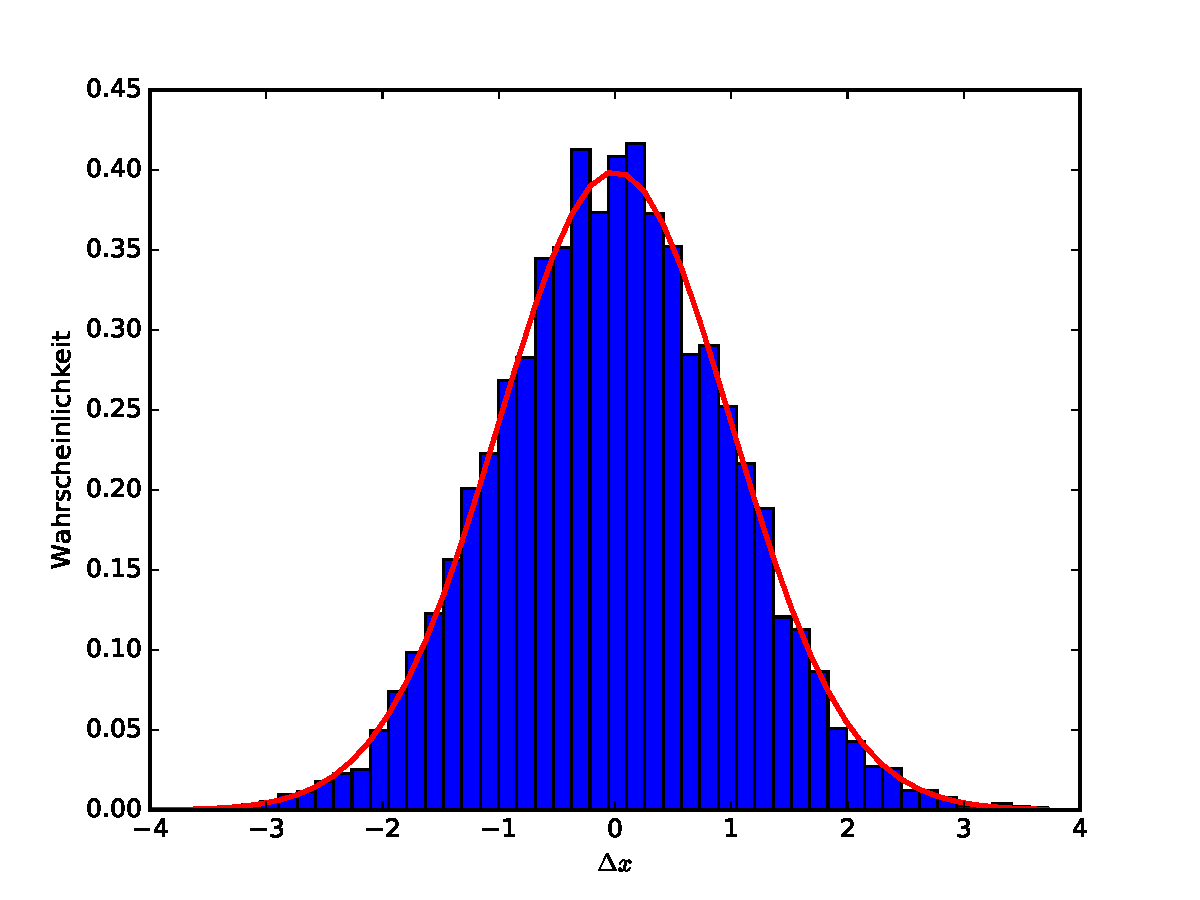
\includegraphics[width=0.7\textwidth]{figures/histogram}
  \caption{Histogram und zugehörige Normalverteilung}\label{fig:histo}
\end{figure}
Um diese Hilfsmittel effizient auf die Brownsche Bewegung anwenden zu können, muss sie noch formal beschrieben werden. Dazu eignet sich das Model eines \textbf{random walks}. Ein \emph{random walk} in einer Dimension funktioniert folgendermaßen: In regelmäßigen Zeitabständen $\tau$ wird eine Münze geworfen. Zeigt sie Kopf bewegt sich das Teilchen einen Schritt nach rechts und zeigt sie Zahl einen Schritt nach links. Die Schrittweite $\delta$ ist für beide Fälle gleich groß. Um die Bewegung zu charakterisieren kann die Diffusionskonstante $D$ definiert werden
\begin{equation}
  D = \frac{\delta^2}{2 \tau}. \label{eq:diff_random}
\end{equation}
Sie gibt an, wie weit sich das Teilchen durch die zufällige Bewegung im Durchschnitt nach einem Schritt von der Nulllage entfernt.\\
Es ist intuitiv klar, dass sich das Teilchen im Durchschnitt nicht von seiner Ursprungslage wegbewegt, ist der Ursprung bei $\Delta x = 0$, dann ist also $\mean{\Delta x} = 0$. Aber was ist mit der Standardabweichung? Da hier $x^2$ eine Rolle spielt, löschen sich die Schritte nach links und rechts nicht gegenseitig aus.
Desto größer die Schrittweite ist, desto weiter wird sich das Teilchen im Durchschnitt von der Nulllage entfernen. Alternativ kann auch die Zeit zwischen zwei Schritten verringert werden. Aus dieser Überlegung ergibt sich die Diffusionskonstante $D$ für den Versuch, denn die Diffusionskonstante aus (\ref{eq:diff_random}) beschreibt nur den \emph{random-walk}.\\
Um sie benutzen zu können müsste die durchschnittliche Zeit zwischen den Stößen und die durchschnittliche Verschiebung nach einem Stoß bekannt sein. Diese Größen können aber nicht experimentell ermittelt werden. Stattdessen kann die Verschiebung zwischen zwei Messungen als \emph{random-walk} aufgefasst werden. Die Schrittweite dieses \emph{random-walks} ist nicht konstant, aber wenn die Bewegung genügend lange beobachtet wird, kann die mittlere Verschiebung als Schrittweite $\delta$ gewählt werden. Das ist aber gerade die Standardabweichung $\sigma$ der Verschiebung $\Delta x$. Und die Zeit zwischen zwei Schritten ist die Zeit zwischen zwei Messungen $t$. Damit ist die experimentell ermittelte Diffusionskonstante
\begin{equation}
  D = \frac{\sigma^2}{2 t}. \label{eq:diff}
\end{equation}
Sie gibt an, wie weit sich das Teilchen in einer Zeit $t$ im Durchschnitt von seinem Ursprung entfernt.\\

Wird der \emph{random walk} nur eine kurze Zeit beobachtet, können aufgrund der zufälligen Natur keine genauen Aussagen gemacht werden. Erst für lange Zeitreihen werden sich die Messwerte an die theoretischen Werte annähern. Alternativ können aber auch viele \emph{random walks} für kurze Zeit betrachtet werden. Das ist das \textbf{Ergodentheorem}. Es besagt, dass es für zufällige thermodynamische System äquivalent ist, ein System über lange Zeit zu mitteln, oder viele Systeme über kurze Zeit. In dem Experiment wird eine lange Brownsche Molekularbewegung beobachtet, zur Auswertung muss sie aber in viele kleine Abschnitte zerlegt werden. Das Ergodentheorem ermöglicht es die lange Bewegung mit den vielen kleinen gleich zu setzen.\\
Bei einem \emph{random walk} in zwei Dimensionen, wie er in dem Versuch gemessen wird, können die beiden Richtungen unabhängig voneinander, als zwei \emph{random walks}, betrachtet werden. Es werden also gleichzeitig zwei Münzen geworfen, eine für die Bewegung nach links und rechts und eine für die Bewegung nach oben und unten.\\


Damit kann die Brownsche Bewegung beschrieben werden. Es fehlt aber noch der Zusammenhang zwischen ihr und der thermischen Energie der Flüssigkeit. Die thermische Energie der umgebenden Flüssigkeitsmoleküle führt zu der Bewegung, dass heißt, die thermische Energie der Flüssigkeit ist gleich der Bewegungsenergie. Diese setzt sich zusammen aus der Diffusion und der Reibung des Teilchens in der Flüssigkeit. Die entstehende Gleichung heißt die  \textbf{Einstein-Smoluchowski} Gleichung.
\begin{equation}
  D C = k_B T \label{eq:einstein}
\end{equation}
Dabei ist $k_B$ die Boltzmann-Konstante, $T$ die Temperatur in K und $C$ die Stokessche Reibungskonstante. Die Reibungskonstante gibt an, wie stark die Reibung auf eine Kugel mit Radius $r$ in einer Flüssigkeit mit Viskosität $\eta$ wirkt.
\begin{equation}
  C = 6 \pi \eta r
\end{equation}
In der Einstein-Smoluchowksi Gleichung taucht wieder die Diffusionskonstante auf. Allerdings wird bei der Herleitung in Gleichung (\ref{eq:einstein}) nicht direkt von einem \emph{random walk} ausgegangen. Das $D$ kommt hier von der Diffusionsgleichung
\begin{equation}
  \frac{\partial c}{\partial t}(x, t) = D \frac{\partial^2 c}{\partial x^2} (x, t). \label{eq:diffusion}
\end{equation}
Diese Gleichung beschreibt die zeitliche Änderung der Konzentration $c$, abhängig von ihrer räumlichen Verteilung. Eine konstante Lösung der Diffusion ist es, dass sich die Konzentration solange ändert, bis sie überall gleich ist. Die Geschwindigkeit dieser Änderung ist durch die Diffusionskonstante gegeben.\\
Es lässt sich zeigen, dass die Diffusionskonstante des \emph{random walks} genau der Diffusionskonstante der Thermodynamik entspricht, was auf die enge Verbindung zwischen dem \emph{random walk} und der Brownschen Bewegung hindeutet.
